\section{材料組織の観察}
材料の諸性質及び強度特性等の変化を理解するためには,材料の内部組織を詳しく調べる必要がある.たとえば,手近にある金属を肉眼または顕微鏡で調べてみても,切削加工などによる傷は見えるが,金属組織そのものは見ることはできない.そこで,金属表面が滑らかになるように研磨したのち化学溶液に浸すと,腐食によって組織が凹凸となって現れ,観察が可能となる.

\subsection{機械的研磨法と電解研磨法}
機械的研磨法は被研磨面の凸部を切削,塑性変形,磨耗などによって除去し,平滑面を得る方法である.その方法は,観察しようとする面を粗いエメリー紙で磨き,次いで順に細かいエメリー紙で磨く.エメリー紙による研磨が終わったならば次にバフ研磨をする.そのための研磨機は回転円板上にフェルトを固定したもので,その上に懸濁液(アルミナ/ダイアモンドペースト)を振りかけながら試料を軽く押しつけて研磨する.電解研磨法は被研磨面の微小凸部を凹部よりも優先的に溶解させて平滑面を得る方法である.その原理は次の通りである。凹凸のある金属面を化学研磨浴に浸すと,研磨面との界面に溶解反応で生じた金属酸化物の拡散層が形成される.そして,金属はこの拡散層を通して液体中に塩として拡散溶解していく.この段階での拡散速度 $V$は,
\begin{equation}
    V = D(C_e - C_0)/\delta
    \label{eq:diffusion}
\end{equation}
である.ここで,$D$ は拡散速度定数,$\delta$は拡散層の厚さ,$C_0$は化学研磨液中の金属イオン濃度,$C_e$は金属表面上の金属イオン濃度である.式(\ref{eq:diffusion})の拡散層の厚さ$\delta$が見かけの金属表面に対して一様であろうとするならば,凸部は薄く,したがって$V$は速くなり,凹部では厚く,$V$は遅くなるので平滑化が行われる.図\ref{fig:平滑化のモデル}に平滑化のモデルを示す.

本実験では,電気化学的に凸部が陽極に,凹部が陰極に帯電するように試料を設置し,局部電池を形成させながら凸部を溶解させ平滑化を試みる.その概略図を図\ref{fig:電解研磨槽概略図}に示す.また,電解研磨は,図\ref{fig:理想的な電圧電流}に示すCD付近のアノード電位をかけ,酸化被膜の形成と溶解を繰り返し起こさせ表面を研磨する.

\begin{figure}[htbp]
    \centering %中央揃え
    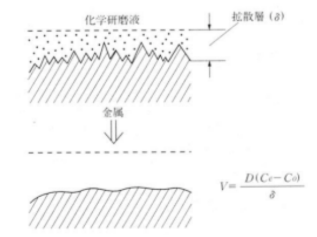
\includegraphics[width=100truemm,clip]{fig/fig_平滑化のモデル.png}
    \caption{Model diagram of smoothing.}
    \label{fig:平滑化のモデル}
\end{figure}

\begin{figure}[htbp]
    \centering %中央揃え
    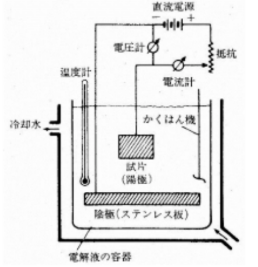
\includegraphics[width=100truemm,clip]{fig/fig_電解研磨槽概略図.png}
    \caption{Electropolishing tank schematic.}
    \label{fig:電解研磨槽概略図}
\end{figure}

\begin{figure}[htbp]
    \centering %中央揃え
    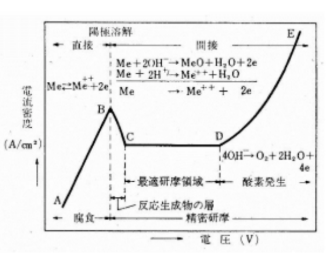
\includegraphics[width=100truemm,clip]{fig/fig_理想的な電圧電流.png}
    \caption{Ideal voltage-current curve.}
    \label{fig:理想的な電圧電流}
\end{figure}

\subsection{エッチング}
研磨により鏡面となった試料を顕微鏡で見ても,金属組織そのものを見ることはできない.そこで,エッチング(etching)を施す.エッチングは,化学的あるいは電気化学的な方法によって組織を現出させる操作である.化学的エッチングは,研磨した試料を腐食液(etchant,etching solution)中に数分間浸して表面を腐食することにより,その内部組織あるいは各結晶粒の方位に応じた凹凸を生じさせる手法である.表\ref{tbl:腐食液の例}に腐食液の代表的なものを示す.酸,アルコールおよび酸化剤からなるものが多い.電気化学的なエッチングは,化学的にエッチングが困難な試料(ステンレス鋼や高合金鋼など)に広く行われている.試料を陽極とし,試料と同等の素材などを陰極とし,試験溶液中で定電位もしくは定電流電解することで所望の組織を現出させる.いずれも,組織に対応した凹凸を試料表面に現出させることで顕微鏡などを用いた組織観察が可能となる.

\begin{table}[htbp]
    \centering
    \caption{Example of corrosive liquid.} % 表のキャプション
    \label{tbl:腐食液の例} % 参照用ラベル
    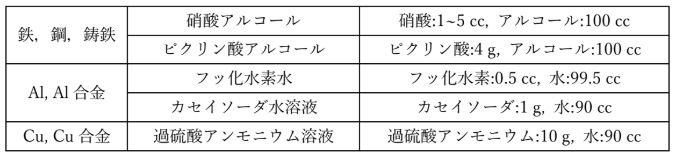
\includegraphics[width=0.8\textwidth]{fig/tbl_腐食液の例.png} % 画像ファイル名と幅を指定
\end{table}